\chapter{Evaluation}\label{chap:evaluation}
In this chapter, we first present our choice of datasets in \autoref{sec:eval:dataset-choice}. As we follow the KDD process, we then lead through the data pre-processing and transformation phases in \autoref{sec:eval:data-preprocessing} and \autoref{sec:eval:data-transformation}. The latter section also covers the strategy used to engineer the features for the SP-2 and PFS models.
The system configuration and the used training strategy is presented in \autoref{sec:eval:test-setup}, followed by the set of criteria by which we judge the results in \autoref{sec:eval:criteria}. Finally, the chapter ends with the presentation in \autoref{sec:eval:results} and discussion of the results in \autoref{sec:eval:discussion}. Used and relevant technologies are highlighted in each section.

Through the use of the framework described in the previous chapter, we can evaluate four different algorithms for next-activity prediction side-by-side: Two implementations that mimic the networks by Evermann et al. and Schönig et al, and the PFS and SP2 approaches presented in \autoref{chap:taking-inspiration}. The reimplementation of Evermann's and Schönig's approaches will be referred to as EVM and SCH respectively. For each model, we will analyze the performance differences between the four different batching strategies from \autoref{chap:training-framework}.

\section{Choice of datasets}
\label{sec:eval:dataset-choice}
In \autoref{sec:intro:contribution}, we criticized the great variety of datasets used to evaluate approaches in Predictive Process Monitoring. While we can not establish a standard, we ensure comparability of our results to a variety of works by evaluating the four models on seven datasets:

\begin{itemize}
    \item BPIC11, an event log from cases in a Gynaecology department of a Dutch Academic Hospital~\cite{BPIC2011}
    \item BPIC12, an event log for loan and overdraft applications from a Dutch Financial Institute~\cite{BPIC2012}
    \item BPIC15 is divided into five logs. Each contains all building permit applications over a period of approximately four years from a Dutch municipality. They are referred to as BPIC15-1 to BPIC15-5 in the following~\cite{BPIC2015}
\end{itemize}

We picked the three BPIC datasets as we believe that they cover a spectrum of process complexity. We take the increasing number of distinct activities and variance in trace length to be indicators of complexity. \autoref{tab:dataset-characteristics} sums up the key properties discussed in the following.

The least complex process is traced in BPIC12, with a small variance in trace length and a very small number of different activities. From BPIC12, process models were also easily mined~\cite{adriansyah2012mining}.

The process in BPIC11 seems to be the most complex, with long traces and an especially high number of distinct activities. Process models were barely obtained from it~\cite{bose2011analysis}.

BPIC15 resides relatively in the middle of the two in terms of complexity. The mined process models from it were more complex than for BPIC12~\cite{van2015benchmarking}.\\

\noindent Additionally, the datasets allow us to compare our findings to the following works, which also worked on next-element predictions. When comparing, it is important to differentiate between the works that focused on case-specific predictions like us and those that focused on whole event streams:

\begin{itemize}
    \item Predicting the next element in a stream, not specific to a case
    \begin{itemize}
        \item BPIC12: Tax et al.~\cite{tax2017}
        \item BPIC12: Evermann et al.~\cite{evermann2016}
    \end{itemize}
    \item Predicting the next element for a specific case
    \begin{itemize}
        \item BPIC12: Böhmer et al.~\cite{boehmer2018probability}
    \end{itemize}
\end{itemize}

\begin{table}
  \centering
  \begin{adjustbox}{center}
  \begin{tabular}{lrrrrrrrr}
  \textbf{Dataset} & \textbf{min $TL$} & \textbf{max $TL$} & \textbf{$\overline{TL}$} & \textbf{$\sigma_{TL}$} & \textbf{Traces} & \textbf{Events} & \textbf{Activities} \\
  \hline
  \textbf{BPIC12}   & 3 & 96  & 12.56 & 11.33 & 13 087 & 164 506 & 23\\
  \textbf{BPIC15-4} & 1 & 116 & 44.91 & 14.63 & 1053 & 47 293 & 356\\
  \textbf{BPIC15-3} & 3 & 124 & 42.35 & 16.05 & 1409 & 59 681 & 383\\
  \textbf{BPIC15-5} & 6 & 154 & 51.10 & 15.82 & 1156 & 59 083 & 389\\
  \textbf{BPIC15-1} & 2 & 101 & 43.55 & 16.74 & 1199 & 52 217 & 398\\
  \textbf{BPIC15-2} & 1 & 132 & 53.31 & 20.32 & 832 & 44 354 & 410\\
  \textbf{BPIC11}  & 1 & 1 814& 131.49&194.01 & 1 143 & 150 291 & 524
  \end{tabular}
  \end{adjustbox}
  \caption[Trace properties in each dataset]{Properties of the traces contained in the used datasets, sorted by activity count. $TL$ abbreviates trace length}
  \label{tab:dataset-characteristics}
\end{table}

\section{Data pre-processing}
\label{sec:eval:data-preprocessing}
In the first step of the KDD process~\cite{fayyad1996data}, the data is pre-processed to prepare the data for a data mining use case and eliminate generally known properties that hinder machine learning model performance. In our case, this encompassed three steps for all datasets:

\begin{enumerate}
    \item Filter for completed events
    \item Drop all columns which exhibit zero entropy, i.e. which contain only a single value
    \item Eliminate features which correlate strongly. To account for categorical correlation, the bias-corrected version of Cramér's~V~\cite{bergsma2013bias} is used.
\end{enumerate}

In step 1, the \verb=lifecycle:transition= feature was filtered so that only completed events were left. This was done to reduce dimensionality and improve comparability because BPIC11 only contains completed events.

In step 2, the \verb=lifecycle:transition= feature was removed in every dataset since it had been filtered before. No other features exhibited zero entropy.

In step 3, the results from the pairwise application of Cramér's~V~\cite{bergsma2013bias} on the features in a dataset reveal that some features correlate strongly with several others in the BPIC11 and BPIC15 datasets. The respective heatmaps can be found in \autoref{appendix:correlation-heatmaps}. Thus, these were dropped. As evidenced in the respective heatmap, the BPIC12 dataset with its small number of features did not require any removals. \autoref{tab:dataset-preprocessing} summarizes which features were removed and which ones were kept after the three steps.

\begin{table}[!htb]
\centering
\begin{adjustbox}{center}
\begin{tabular}{lp{6cm}p{6cm}}
\textbf{Dataset} & \textbf{Omitted features} & \textbf{Remaining features}\\
\hline
\textbf{BPIC11} & \verb=lifecycle:transition=, \verb=Producer code=,  \verb=Activity code=,  \verb=Specialism code= & \verb=time:timestamp=, \verb=concept:name=, \verb=org:group=, \verb=Number of executions=, \verb=Activity code=, \verb=Producer code=, \verb=Specialism code=, \verb=Section=\\
\textbf{BPIC12} & \verb=lifecycle:transition= & \verb=org:resource=, \verb=concept:name=, \verb=time:timestamp=\\
\textbf{BPIC15} & \verb=lifecycle:transition=, \verb=activityNameNL=, \verb=activityNameEN=, \verb=action_code=, \verb=dueDate= & \verb=time:timestamp=, \verb=dateFinished=, \verb=planned=, \verb=concept:name=, \verb=monitoringResource=, \verb=org:resource=,     \verb=question=
\end{tabular}
\end{adjustbox}
\caption{Omitted features during pre-processing}
\label{tab:dataset-preprocessing}
\end{table}

The activities described above were conducted in JupyterLab notebooks~\cite{web:jupyter}, where Anaconda~\cite{web:anaconda} was used to create a stable development environment. The OpyenXes~\cite{web:opyenxes} library proved to be especially useful for transferring raw XES logs into workable Pandas data frames.

\section{Data transformation}
\label{sec:eval:data-transformation}
After selecting suitable features in the first step, the second step of the KDD process~\cite{fayyad1996data} suggests the transformation of the remaining features into representations that are better received by predictive models. Also, feature engineering is part of this step, and so the construction of the SP-2 and PFS features is explained in the following subsections.

\subsection*{Transforming basic features}
The features remaining after selection can be divided into three categories: timestamps, numerical and categorical. The transformation applied to each category of feature is described briefly in the following:

Timestamps are converted to numerical features for each trace, i.e. each timestamp $t_i$ is made relative to the beginning of a trace by replacing it with the result of $t_i - t_0$. Relative timestamps have been shown to work with sequential data~\cite{lessmannBADS}.

Each numerical feature $x$ is normalized using the min-max method with min- and max-values specific to each trace. This also includes the relative timestamps. For those traces that contain only a single timestamp, an edge case is introduced:

$$normalize(x) =
\begin{cases}
\frac{x-min(x)}{max(x)-min(x)} & \text{if } min(x) \neq max(x)\\
1 & \text{otherwise}
\end{cases}
$$

Categorical features were encoded using one-hot encoding, since no ordinal relationships were present in the data, and the dimensions were not too large.

\subsection*{Engineering the SP-2 features}
SP-2 features were proposed in the SPiCe submission by Shibata et al.~\cite{shibata2016bipartite}. In a binary bag-of-words feature vector, they mark whether an activity has occurred in the past. As such, these features are engineered in an iterative fashion. \autoref{lst:sp2-generation} shows the construction of the feature vector in Python.

For every trace, a new feature vector \texttt{sp2\_df} is created and the occurrence of the first activity, contained in the column \verb=target_col=, is marked inside it. Then, a loop begins over the remaining steps, where each previous row inside \texttt{sp2\_df} is copied into the currently indexed row and the presence of the current activity is marked. This repeats itself until the trace has been processed completely, leaving behind a complete SP-2 feature vector for a trace.

\begin{listing}[ht]
\begin{minted}[linenos]{python}
# Dataframe initialization with zeroes
sp2_df = pd.DataFrame(columns=activity_labels,
                      index=range(0,len(t)),
                      dtype=np.bool)
for col in sp2_df.columns: sp2_df[col].values[:] = 0

# mark first occuring activity
cname = "{0}{1}".format(sp2_prefix, t[target_col][0])
sp2_df[cname].values[0]  = 1

# copy over values from last row and
# set activity labels accordingly
for i in range(1,len(t)):
    first_activity_name = t[target_col].iloc[i]
    col = "{0}{1}".format(sp2_prefix,first_activity_name)

    sp2_df.values[i] = sp2_df.values[i-1]
    sp2_df[col].values[i] = 1
\end{minted}
\caption{Generating SP-2 features for a single trace \texttt{t} and a specific target column \texttt{target\_col}.}
\label{lst:sp2-generation}
\end{listing}

\FloatBarrier
\subsection*{Engineering the PFS features}
As presented in \autoref{sec:contrib:pfs-inspiration}, PFS features encode subsequence occurrence. Klinkmüller et al. claim that these features can help models cover a broader variety of relationships~\cite{klinkmuller2018reliablemonitoring}.

The features for the PFS model were created with the help of the PrefixSpan algorithm implementation from the \textit{prefixspan-py} library~\cite{web:prefixspan-py}. Similarly to the SP-2 features, they are based on the target variable.

As \autoref{lst:pfs-mining} shows, prefixspan-py greatly facilitates obtaining subsequences. The depicted function call returns the top 25 closed subsequences ranked by their support metric. Mined from the entirety of traces, these subsequences are picked as features to be encoded. By choosing 25, we stay well above the minimum support requirement of $0.05$ chosen by Klinkmüller et al.~\cite{klinkmuller2018reliablemonitoring}.

\begin{listing}[ht]
\begin{minted}[linenos]{python}
prefixspan_traces = PrefixSpan(encoded_traces)
closed_sequences = prefixspan_traces.topk(25, closed=True)
\end{minted}
\caption{Obtaining closed sequences using the \textit{prefixspan-py} library.}
\label{lst:pfs-mining}
\end{listing}

After mining the sequences, a loop is executed for every trace - shown in \autoref{lst:subsequence-feature-creation}. This loop constructs the PFS feature vector in an iterative fashion.

For each index \verb=i= it is checked whether any of the mined subsequences starts at that position. This is checked by peeking ahead of \verb=i= for the length of the subsequence. As in the case of the SP-2 features, the occurrence of a subsequence is marked with a boolean flag in the feature vector \verb=subseq_df= from the row that it occurred in onwards.

\begin{listing}[ht]
\begin{minted}[linenos]{python}
# Initialize the feature vector
# subsequences have not happened yet
subseq_df = pd.DataFrame(columns=subseq_labels,
                         index=range(0,len(t)),
                         dtype=np.bool)
subseq_df[:].values[:] = False
tlen = len(t)

# Dictionary encode activity names, entire trace
activity_codes = t[target_col].map(name_to_int)

for i in range(0, tlen):
  # loop through all subsequences
  for subseq_idx, subseq in enumerate(ps):
    if tlen <= i+len(subseq): continue

    # check if subsequence starts at offset j+i
    # abort at first mismatch
    subsequence_found = True
    j = 0

    while subsequence_found and j < len(subseq):
      if subseq[j] != activity_codes[j+i]:
        subsequence_found = False
        j += 1

    # if subseq took place, subsequence_found is still true
    if subsequence_found:
      subseq_df.values[j+i:,subseq_idx] = True
\end{minted}
\caption{Enriching a trace \texttt{t} with subsequence features by detecting those that are contained inside it.}
\label{lst:subsequence-feature-creation}
\end{listing}

\subsection*{Constructing prediction labels}
For each event $e_t$ at a given timestep $t$, the prediction label $\#_{activity name}(e_{t+1})$ was constructed, essentially picking the activity name from the following event. For the target of the final event of a trace, a marker for denoting the end of the sequence, \verb=EOS=, was introduced.

To finally work with the data, the column containing the name of the next activity needed to be identified for each dataset. The XES standard defines that this column is called \verb=concept:name=~\cite{Aalst2016}.

\subsection*{Splitting the datasets}
To verify model performance on unseen data, a portion of the dataset is often put aside for testing purposes~\cite{kuhn2013applied}.

We split all datasets into training and validation sets of complete traces. While $25\%$ of the traces were used for validation, the remaining $75\%$ were used for training purposes. The traces were shuffled and stratified to contain an approximately similar distribution of trace lengths. This avoids possible biases towards trace lengths. The event order in a trace was not changed.

\section{Training configuration}\label{sec:eval:test-setup}
This section highlights the model configuration, and the employed hyper-parameters for each model, as well as batch sizes of each batching strategy.

We made use of the framework described in \autoref{chap:training-framework}, which implements early stopping, and saves model snapshots when its validation loss hits a new record low. If the validation loss did not improve for 10 epochs, the training was stopped.

The implementation of the padding strategy required a small cue: The padding values incurred a large memory overhead so that BPIC11 could not fit into GPU memory. For this reason, we filtered out $20\%$ of the longest traces. With regard to the length distribution in \autoref{fig:bpic2011-length-distribution}, these seem to be strong outliers.

The models themselves were trained with different optimizers, and various initialization strategies for weights, depending on the original author's choice~\cite{evermann2016, schoenig2018}. \autoref{tab:model-setup} shows these hyper-parameters per network side-by-side and recapitulates the used event attributes. The batch size is also an important hyper-parameter. It depends on the respective batching strategy and is shown in \autoref{tab:batch-sizes}.

\begin{table}[ht!]
\centering
\begin{tabular}{lcccc}
\textbf{Network}&\textbf{EVM}&\textbf{SCH}&\textbf{SP2}&\textbf{PFS}\\
\hline
\textbf{Optimizer} & SGD & \multicolumn{3}{c}{RMSprop} \\
\textbf{Loss}      &\multicolumn{4}{c}{Categorical crossentropy}\\
\textbf{Weight initializer} & Zeros & None & \multicolumn{2}{c}{Glorot normal}\\
\textbf{Epochs}    & 50 & 100 & 150 & 150\\
\textbf{Features}  & \makecell{Activity +\\Resource} & \multicolumn{3}{c}{All event attributes}\\
\end{tabular}
\caption[Used hyper-parameters for each model]{Used hyper-parameters for each model, with the number of epochs to be understood as the maximum number of epochs, as training may stop early}
\label{tab:model-setup}
\end{table}

To conduct the experiments, Docker containers were built with the development Anaconda environment inside them~\cite{web:docker}. Using a version of Docker for GPU applications running on NVIDIA hardware~\cite{web:nvidia-docker}, each network-batch-formatting combination was trained and evaluated on a single NVIDIA K80 GPU. The HPI FutureSOC Lab~\cite{web:fsoc} provided the computational infrastructure and multiple GPUs so that multiple models could be trained and evaluated simultaneously. The complete source code used for evaluation is publicly available on GitHub at \href{https://github.com/flxw/master-thesis-code}{github.com/flxw/master-thesis-code}.

\begin{table}
\centering
\begin{tabular}{c|rrrr}
Dataset & Individual & Grouped & Padded & Windowed \\
\hline
BPIC11    & 1 & $2.80 , \sigma 4.99$ & 7 & 1054\\
BPIC 12   & 1 & $129.14 , \sigma 333.58$ & 89 & 939\\
BPIC 15-1 & 1 & $10.33 , \sigma 11.45$ & 9 & 365\\
BPIC 15-2 & 1 & $6.17 , \sigma 7.57$ & 5 & 316\\
BPIC 15-3 & 1 & $12.27 , \sigma 19.28$ & 10 & 414\\
BPIC 15-4 & 1 & $9.17 , \sigma 14.59$ & 8 & 334\\
BPIC 15-5 & 1 & $9.52 , \sigma 14.36$ & 7 & 420\\
\end{tabular}
\caption[Batch sizes for each dataset and strategy]{Traces per batch for the different datasets and batching strategies. Since the grouped batches vary in size, their size is stated as \textit{average} $, \sigma$ \textit{standard deviation}}
\label{tab:batch-sizes}
\end{table}

\section{Evaluation criteria}\label{sec:eval:criteria}
This section presents how we evaluate the performance of the models. We chose to focus on the following three metrics:

\begin{enumerate}
    \item\textbf{Accuracy} - the share of correct next-activity predictions
    \item\textbf{Resource consumption} - the amount of time required during training
    \item\textbf{Stability} - the change in prediction accuracy with trace progression
\end{enumerate}

While the first two criteria target the general usability of each model, the last one permits making a judgment about the stability of the predictions. It is inspired by the works of Francescomarino et al.~\cite{francescomarino2015} and Klinkmüller et al.~\cite{klinkmuller2018reliablemonitoring} and provides an understanding of how the prediction accuracy of a model changes as the process advances. This can facilitate building trust in the model, as indicated in the introduction of the thesis.

\section{Results}\label{sec:eval:results}
The three aforementioned evaluation criteria were applied to each model-batching combination on each dataset, and the results are presented in this section. By criterion, we go through the measurements. Some of the referenced figures are placed in the appendices, due to space reasons.

\subsection*{Accuracy}
The validation accuracy is a good indicator of the prediction performance of any prediction model. We will go over the model accuracies by batching strategy and explain the results. In \autoref{fig:max-accuracies-bpic2011} to \autoref{fig:max-accuracies-bpic2015-5}, the model performances per dataset are presented, grouped by batching strategy. The plots make apparent that only three models perform well consistently and that the batching strategies can have a profound effect on accuracy.\\

% individual batching strategy
The individual batching strategy often results in slightly worse accuracies than the grouped batching strategy. We trace this back to the more frequent adjustment of weights that can lead the loss optimization into local minima~\cite{keskar2016large}. For this strategy, the SCH model always gives the best accuracies.

% grouped batching strategy
The grouped batching strategy generally leads to top performance in lieu with our SP2 model on any dataset except for BPIC11 and BPIC12. On BPIC11, the strategy brings the best accuracy with the PFS model. On BPIC12, it causes the worst accuracies on the dataset. The explanation for this can be found in \autoref{tab:dataset-characteristics} and \autoref{tab:batch-sizes}. The dataset has the highest number of traces, and a relatively even distribution of lengths, resulting in a small standard deviation. This results in too many traces being put in a single batch, causing lost optimization opportunities. With this in mind, the grouping strategy should be enhanced to split batches if they exceed a certain size threshold. Nonetheless, we realized that the mean of the top accuracies of the SCH, SP2 and PFS models is the highest with the grouping strategy. \autoref{tab:strategy-top-accuracies} illustrates these mean accuracies.
%We also realized that the grouping strategy not only contributes to the best accuracies but also that it has a harmonizing effect on the accuracies among the SCH, SP2 and PFS models. This effect is illustrated in \autoref{fig:accuracy-harmonization}. The heatmap shows how the standard deviation between the top accuracies of the three models decreases with the grouping strategy on any dataset.

% padded strategy
The padded strategy leads to consistently good results throughout the datasets and only loses accuracy on the BPIC11 datasets where the training set had to be shrunk because traces exceeded a length threshold.

% windowed strategy
The batching strategies that provide the whole history in one sample consistently see the SCH, SP2 and PFS models on par with at most $0.1$ difference. The windowed batching strategy leads to very different results, depending on the dataset and model. With a window size of three, suggested by Schönig et al., the model does not have many timesteps to learn from in any given sample. However, this loss of information does not impact the SP2 model. We assume that its SP-2 features encode the history that is cut away and thus help it come close to the general maximum accuracy of the dataset with the exception of BPIC11.

Looking at the accuracy of the EVM model across all datasets, it is evident that it is consistently outperformed. We trace the low accuracy back to the application of an Embedding layer, which we suspect to require more data than included in most datasets to improve its internal data representation.
Its accuracy on the BPIC12 dataset represents an exception. The performance jump here corresponds to the small number of activities and a large number of traces in \autoref{tab:dataset-characteristics}, which could help the Embedding learn better. Therefore, we assume that Embeddings need more training data than currently available to become more effective.

\begin{figure}
    \centering
    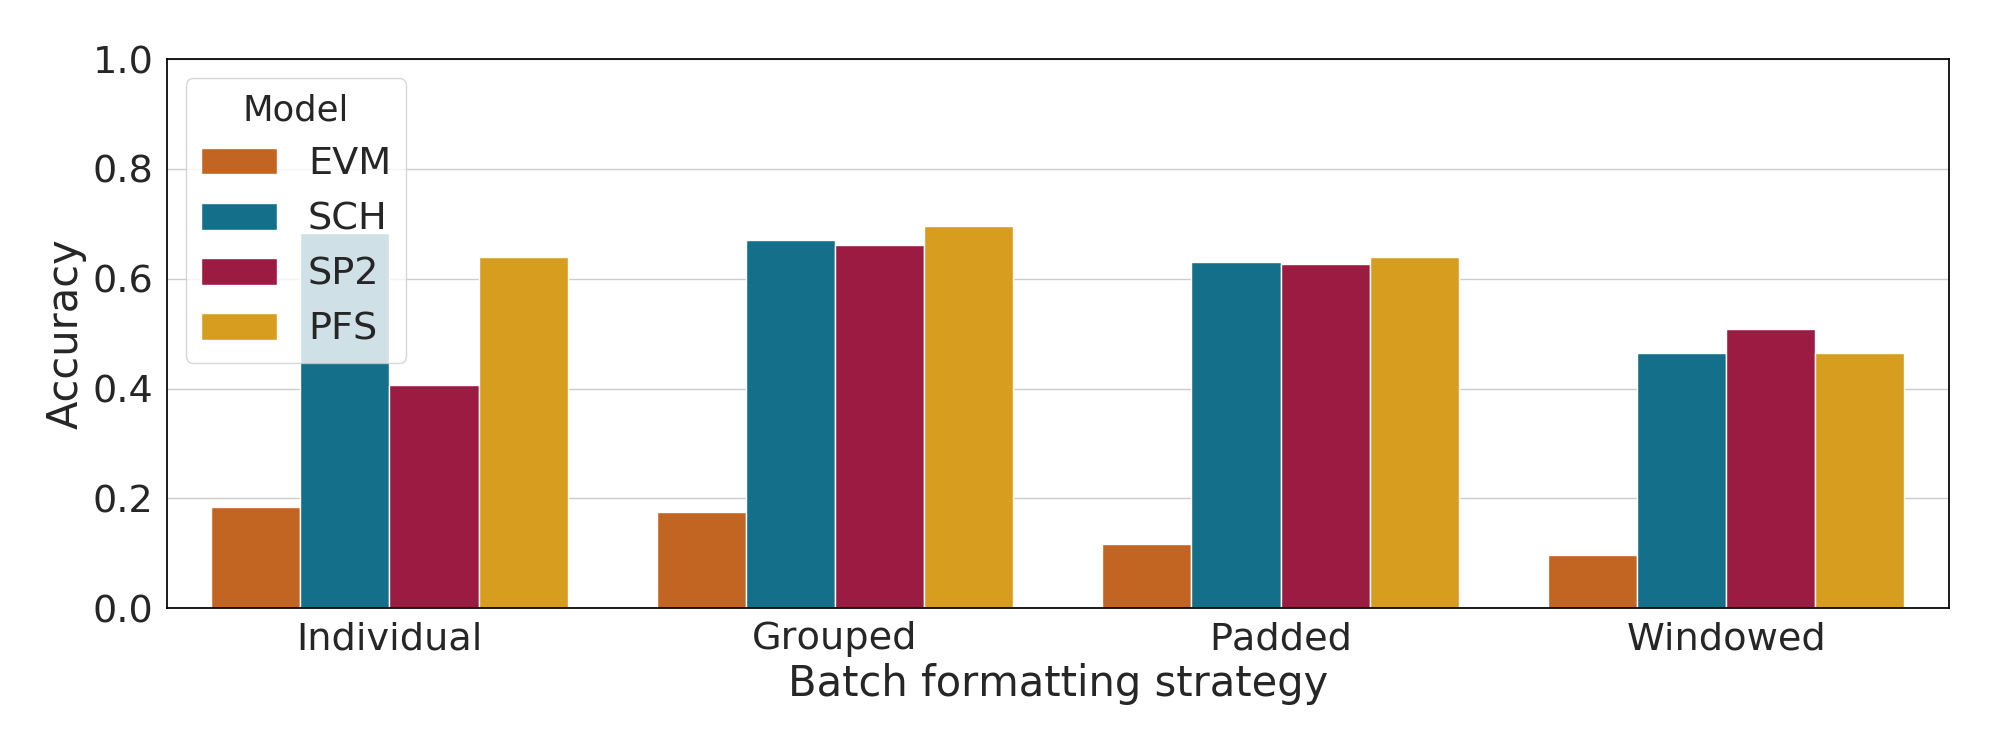
\includegraphics[width=\textwidth]{gfx/bpic2011/accuracies.png}
    \caption{Best accuracies on the validation set of BPIC11}
    \label{fig:max-accuracies-bpic2011}
\end{figure}
\begin{figure}
    \centering
    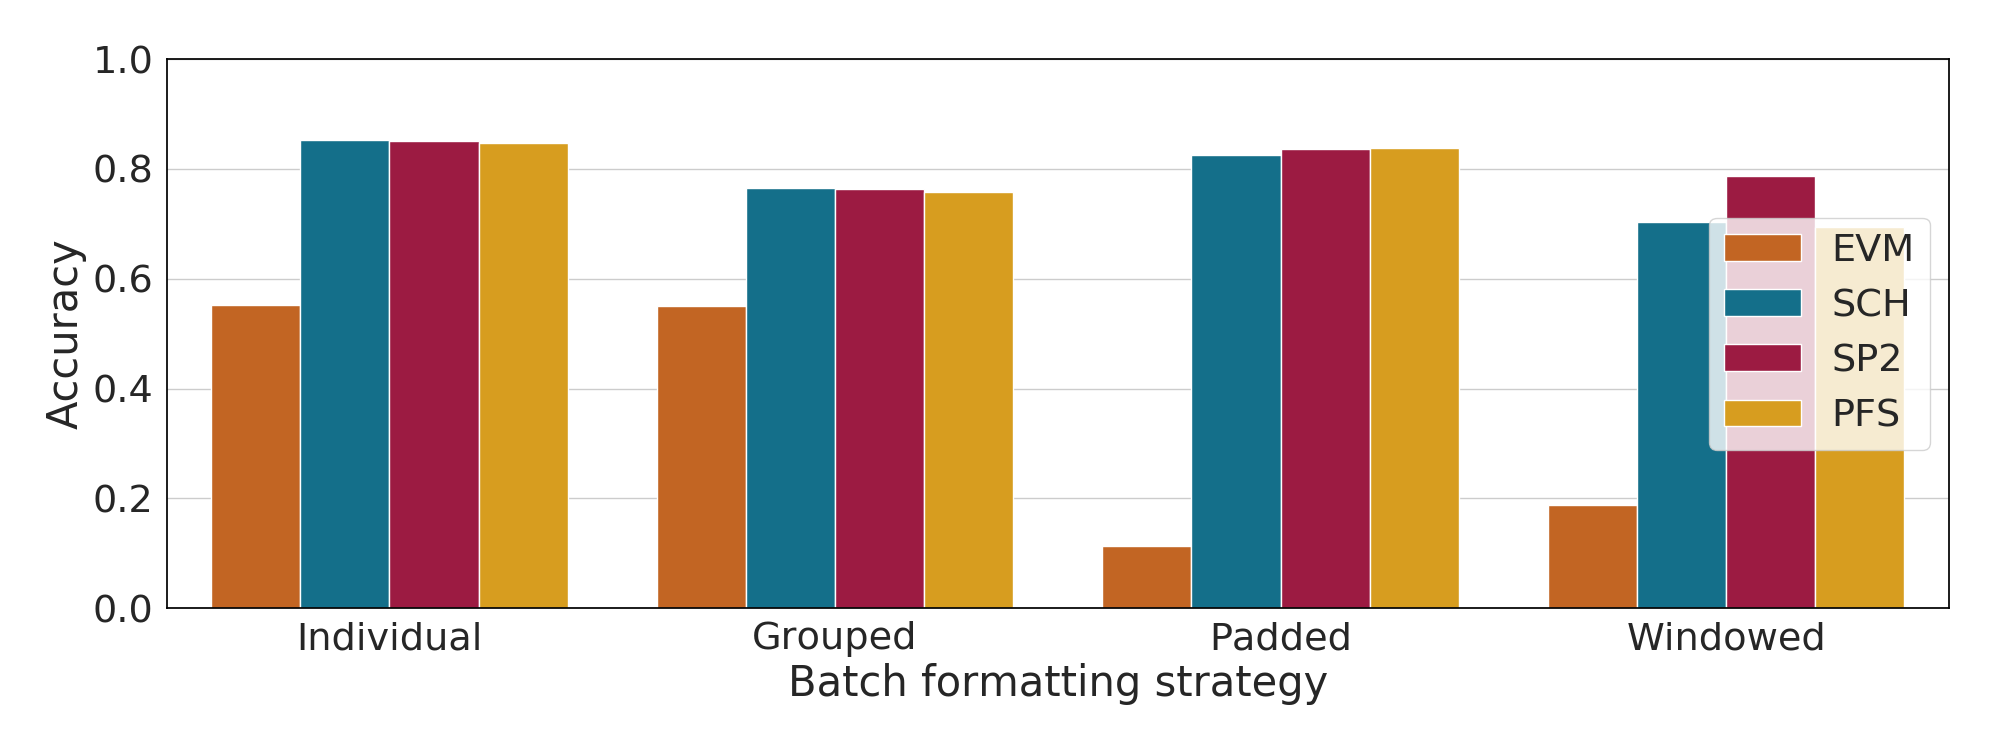
\includegraphics[width=\textwidth]{gfx/bpic2012/accuracies.png}
    \caption{Best accuracies on the validation set of BPIC12}
    \label{fig:max-accuracies-bpic2012}
\end{figure}
\begin{figure}
    \centering
    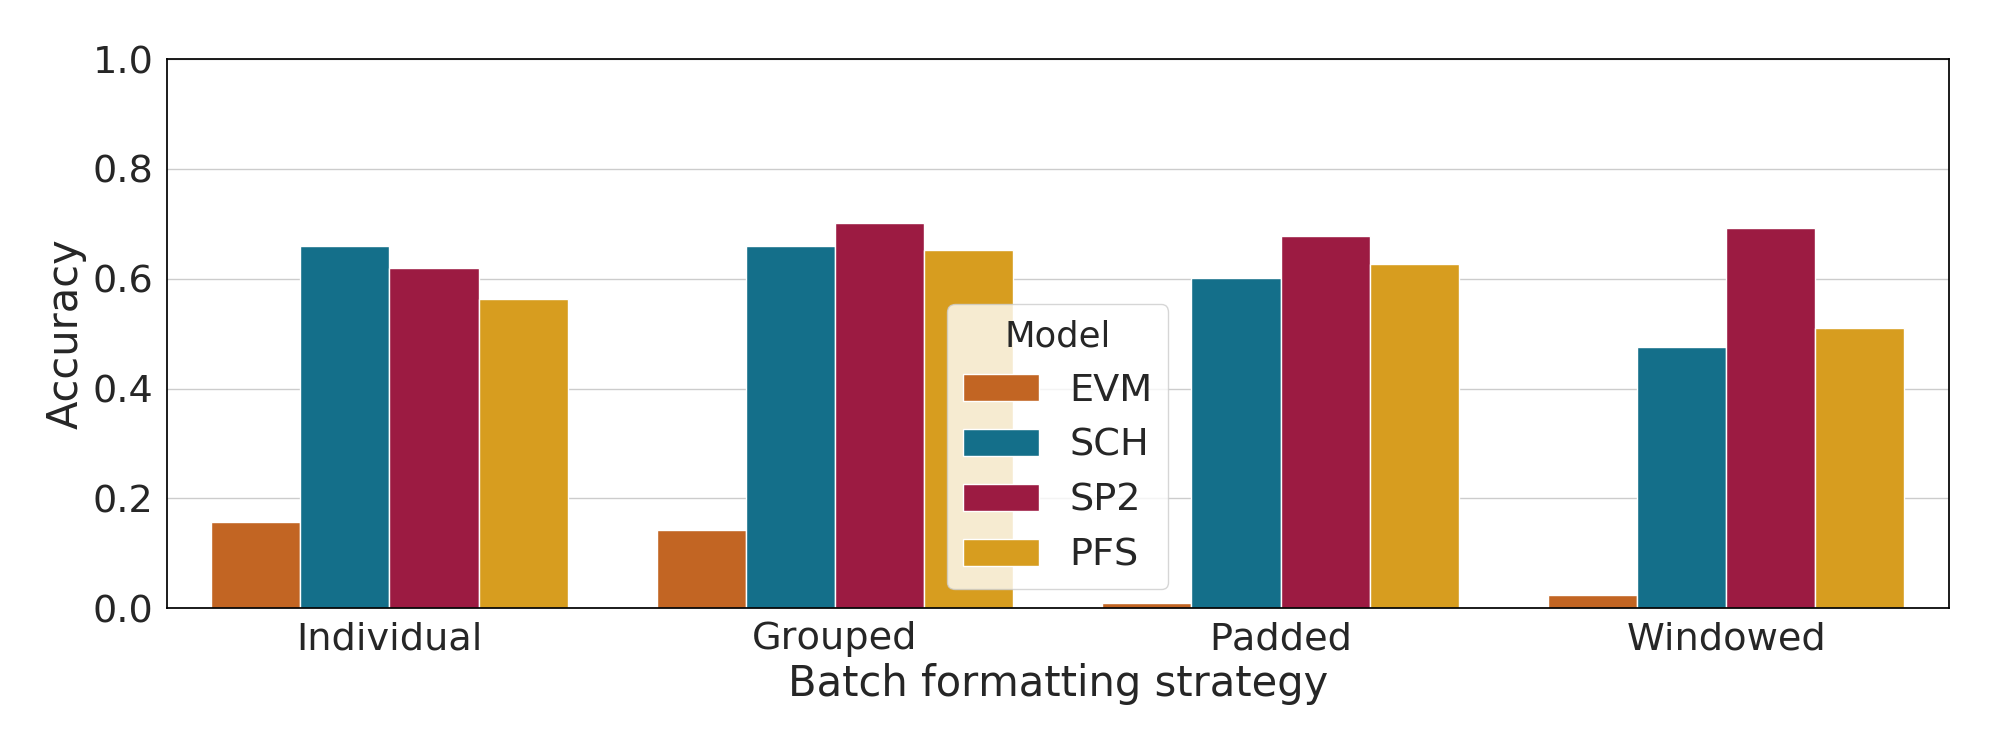
\includegraphics[width=\textwidth]{gfx/bpic2015_1/accuracies.png}
    \caption{Best accuracies on the validation set of BPIC15-1}
    \label{fig:max-accuracies-bpic2015-1}
\end{figure}
\begin{figure}
    \centering
    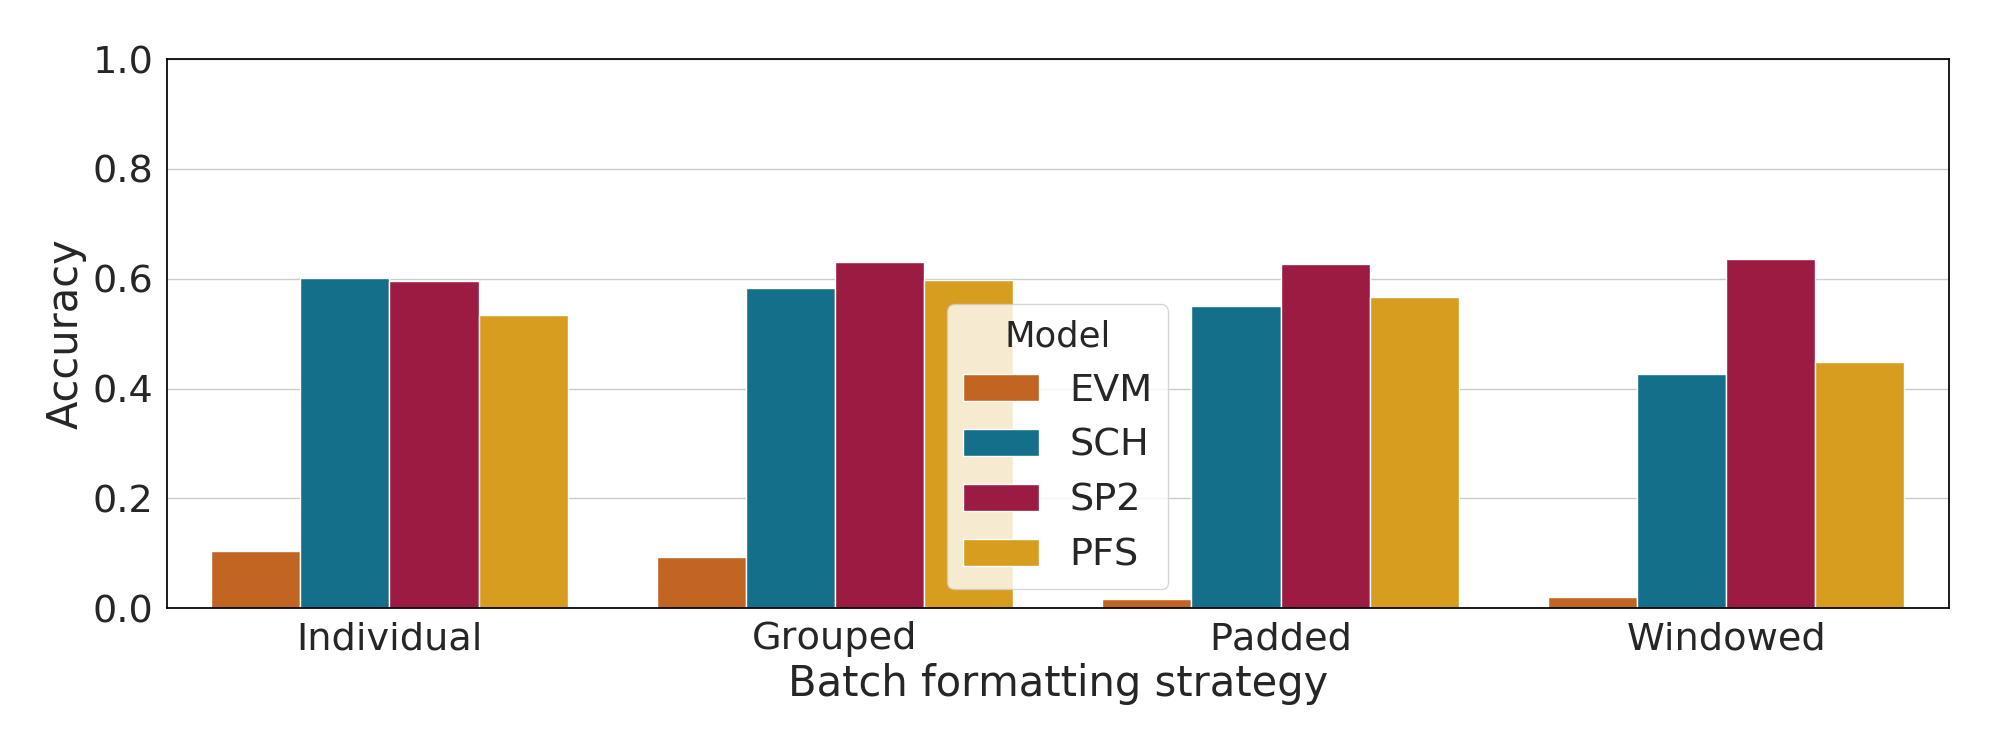
\includegraphics[width=\textwidth]{gfx/bpic2015_2/accuracies.png}
    \caption{Best accuracies on the validation set of BPIC15-2}
    \label{fig:max-accuracies-bpic2015-2}
\end{figure}
\begin{figure}
    \centering
    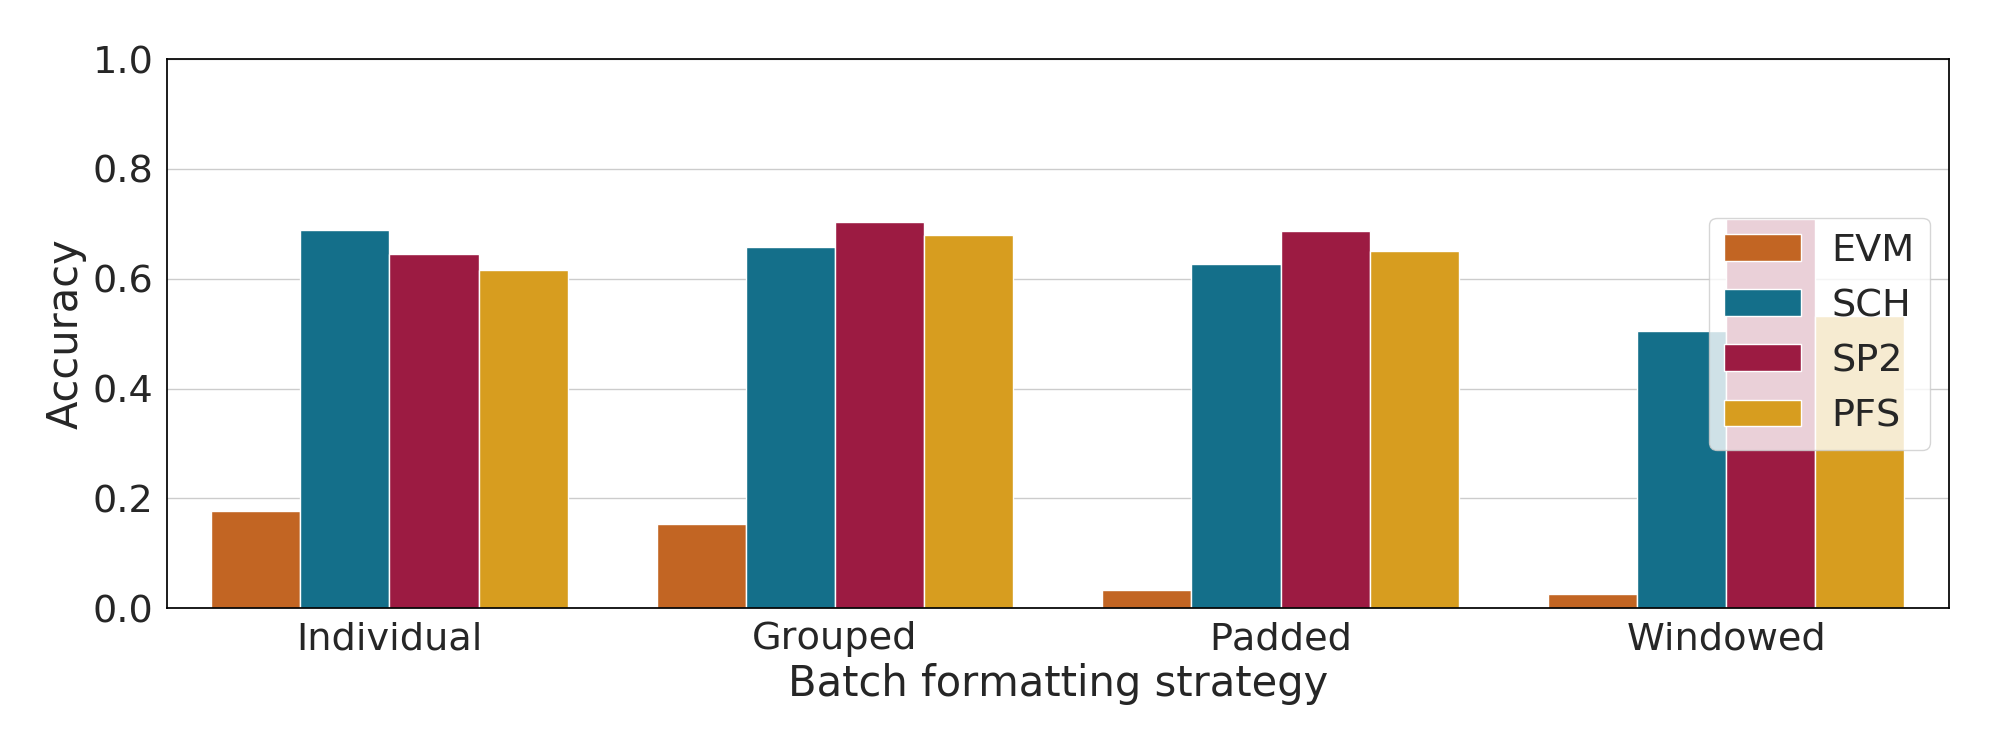
\includegraphics[width=\textwidth]{gfx/bpic2015_3/accuracies.png}
    \caption{Best accuracies on the validation set of BPI15-3}
    \label{fig:max-accuracies-bpic2015-3}
\end{figure}
\begin{figure}
    \centering
    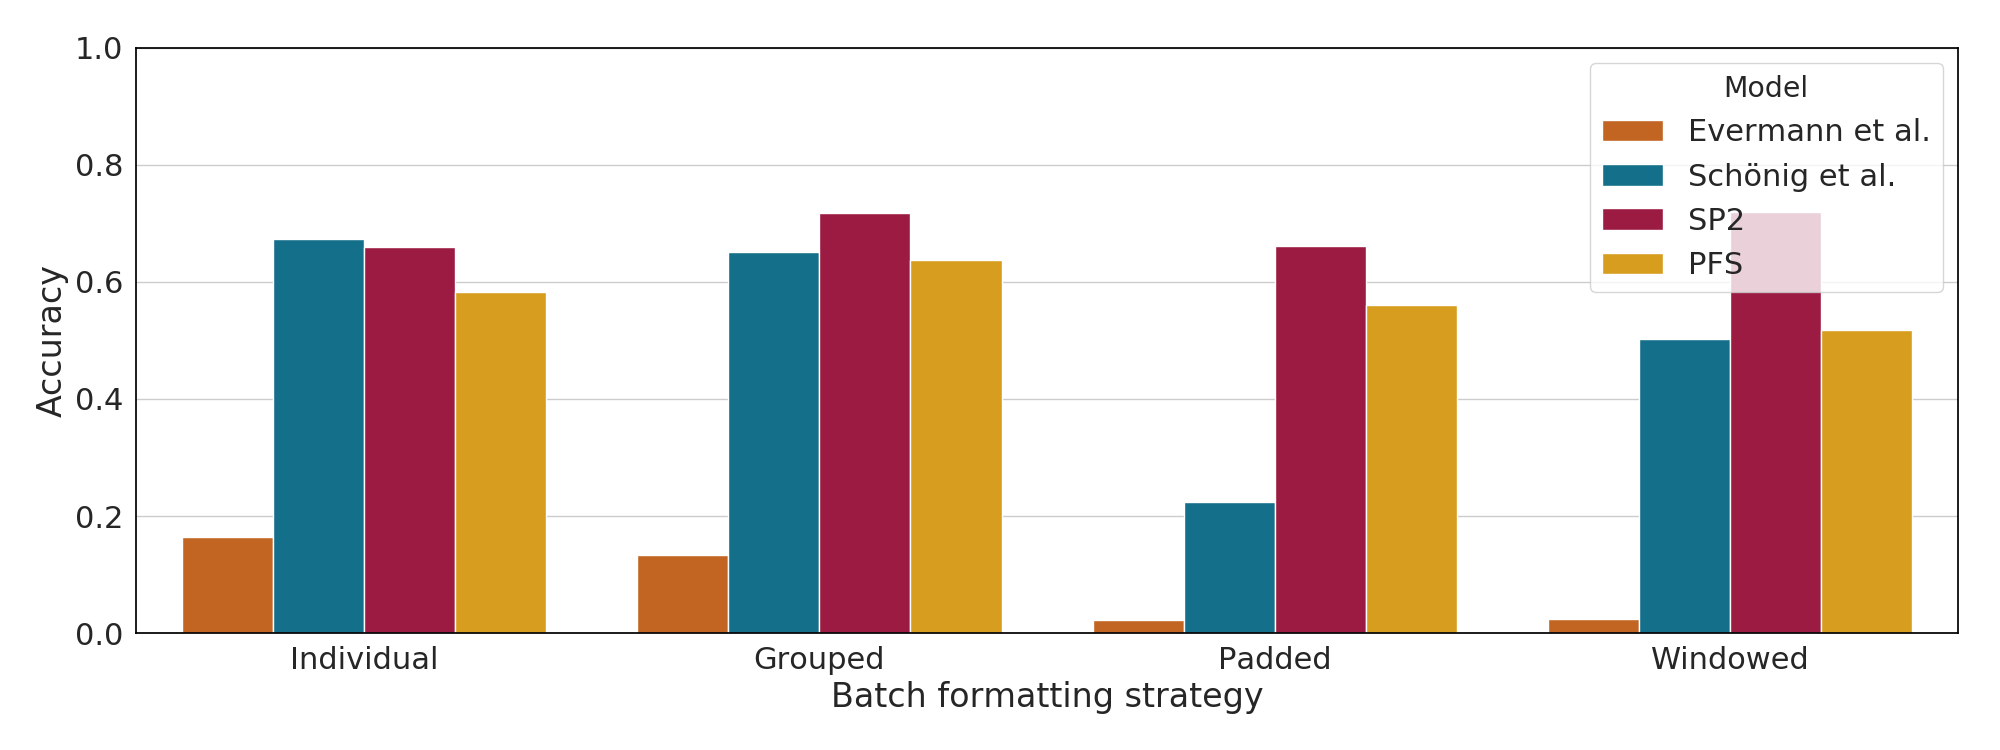
\includegraphics[width=\textwidth]{gfx/bpic2015_4/accuracies.png}
    \caption{Best accuracies on the validation set of BPI15-4}
    \label{fig:max-accuracies-bpic2015-4}
\end{figure}
\begin{figure}
    \centering
    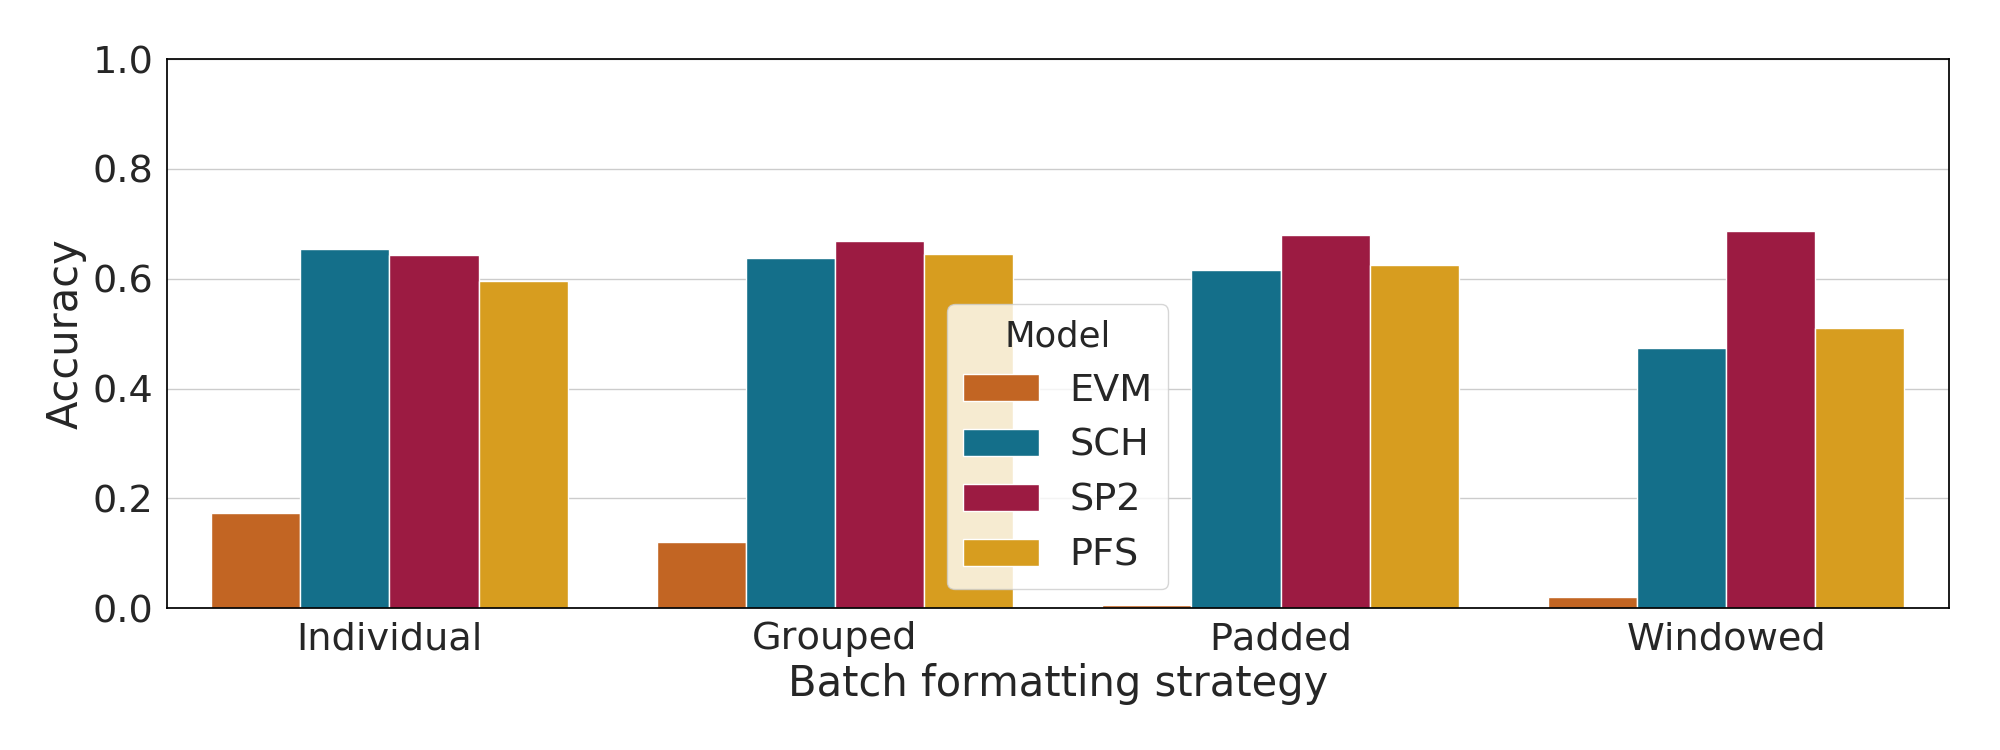
\includegraphics[width=\textwidth]{gfx/bpic2015_5/accuracies.png}
    \caption{Best accuracies on the validation set of BPI15-5}
    \label{fig:max-accuracies-bpic2015-5}
\end{figure}
\begin{figure}
\centering
\begin{tabular}{l|rrrr}
&  Individual &   Grouped &    Padded &  Windowed \\
\midrule
BPIC11   &    0.576469 &  0.676253 &  0.632560 &  0.479481 \\
BPIC12   &    0.850625 &  0.761743 &  0.833241 &  0.728079 \\
BPIC15-1 &    0.614653 &  0.670698 &  0.635351 &  0.559452 \\
BPIC15-2 &    0.577262 &  0.604133 &  0.581127 &  0.503441 \\
BPIC15-3 &    0.649604 &  0.680127 &  0.654643 &  0.581378 \\
BPIC15-4 &    0.638515 &  0.668868 &  0.645301 &  0.579371 \\
BPIC15-5 &    0.630758 &  0.650530 &  0.640852 &  0.557139 \\
\end{tabular}
\caption[Grouping strategy leads to best mean accuracies]{The grouping strategy accuracy mean across the top accuracies of the SCH, SP2 and PFS models is generally the highest}
\label{tab:strategy-top-accuracies}
\end{figure}
\FloatBarrier

\subsection*{Training time}
The training time that a model requires for an epoch is important to gauge the efficiency of its training process. The batch size has a direct effect on the required time since it corresponds to the number of weight adjustments per epoch. \autoref{fig:BPIC11-training-timings} to \autoref{fig:BPIC15-5-training-timings} illustrate the mean time required for training a model for an epoch, grouped by batching strategy. Here, we will go over the training times per batching strategy and explain the results.

Unsurprisingly, the individual batching strategy leads to the longest times overall. \autoref{tab:dataset-characteristics} reveals that this strategy leads to hundreds of weight adjustments per epoch.

The grouped batching strategy leads to significant reductions in training times, depending on how diverse the trace lengths are. \autoref{tab:dataset-characteristics} explains why the reduction is not as big with BPIC11: It exhibits up to 1814 different lengths, while the other datasets only exhibit $5\%$ to $10\%$ of this number.

With the padded strategy, it is possible to overcome the limitations imposed by trace lengths and construct batches out of any number of traces. This makes it easier to optimize the batch size, which can lead to faster training times. That it does not always lead to better accuracies was shown in the previous section, as e.g. this strategy incurs a loss of samples on BPIC11.

Finally, the windowing strategy is the fastest by at least 60 seconds on any dataset. It produces a constant number of timesteps and allows for arbitrary batch sizes.

\begin{figure}
    \centering
    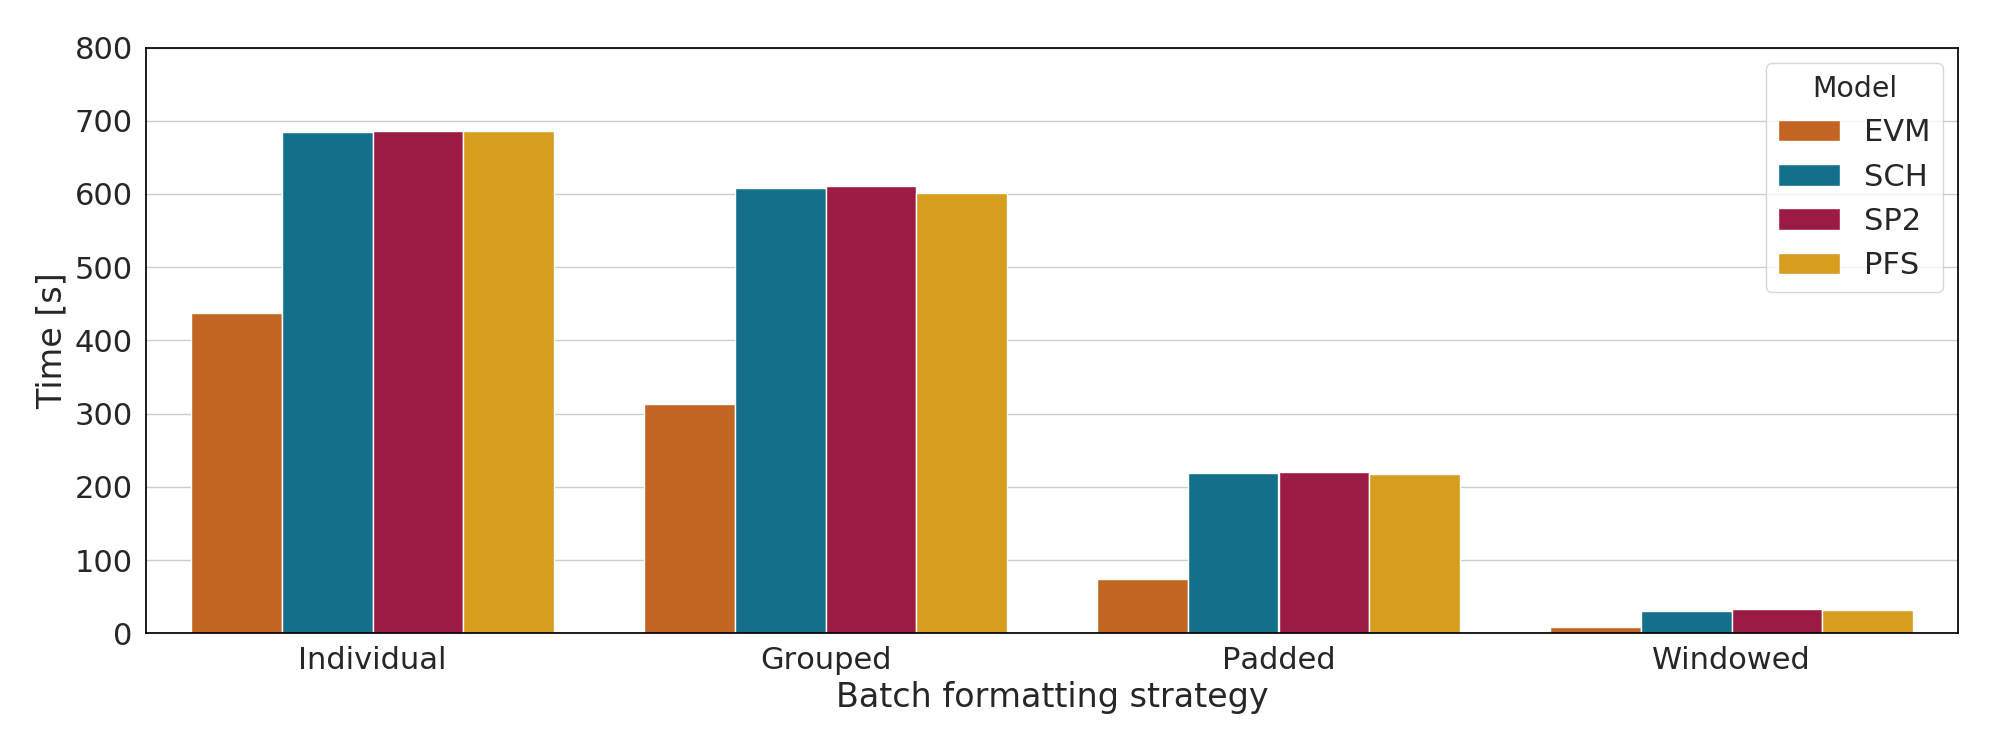
\includegraphics[width=\textwidth]{gfx/bpic2011/train_timings.png}
    \caption{Training times measured on BPIC11}
    \label{fig:BPIC11-training-timings}
\end{figure}
\begin{figure}
    \centering
    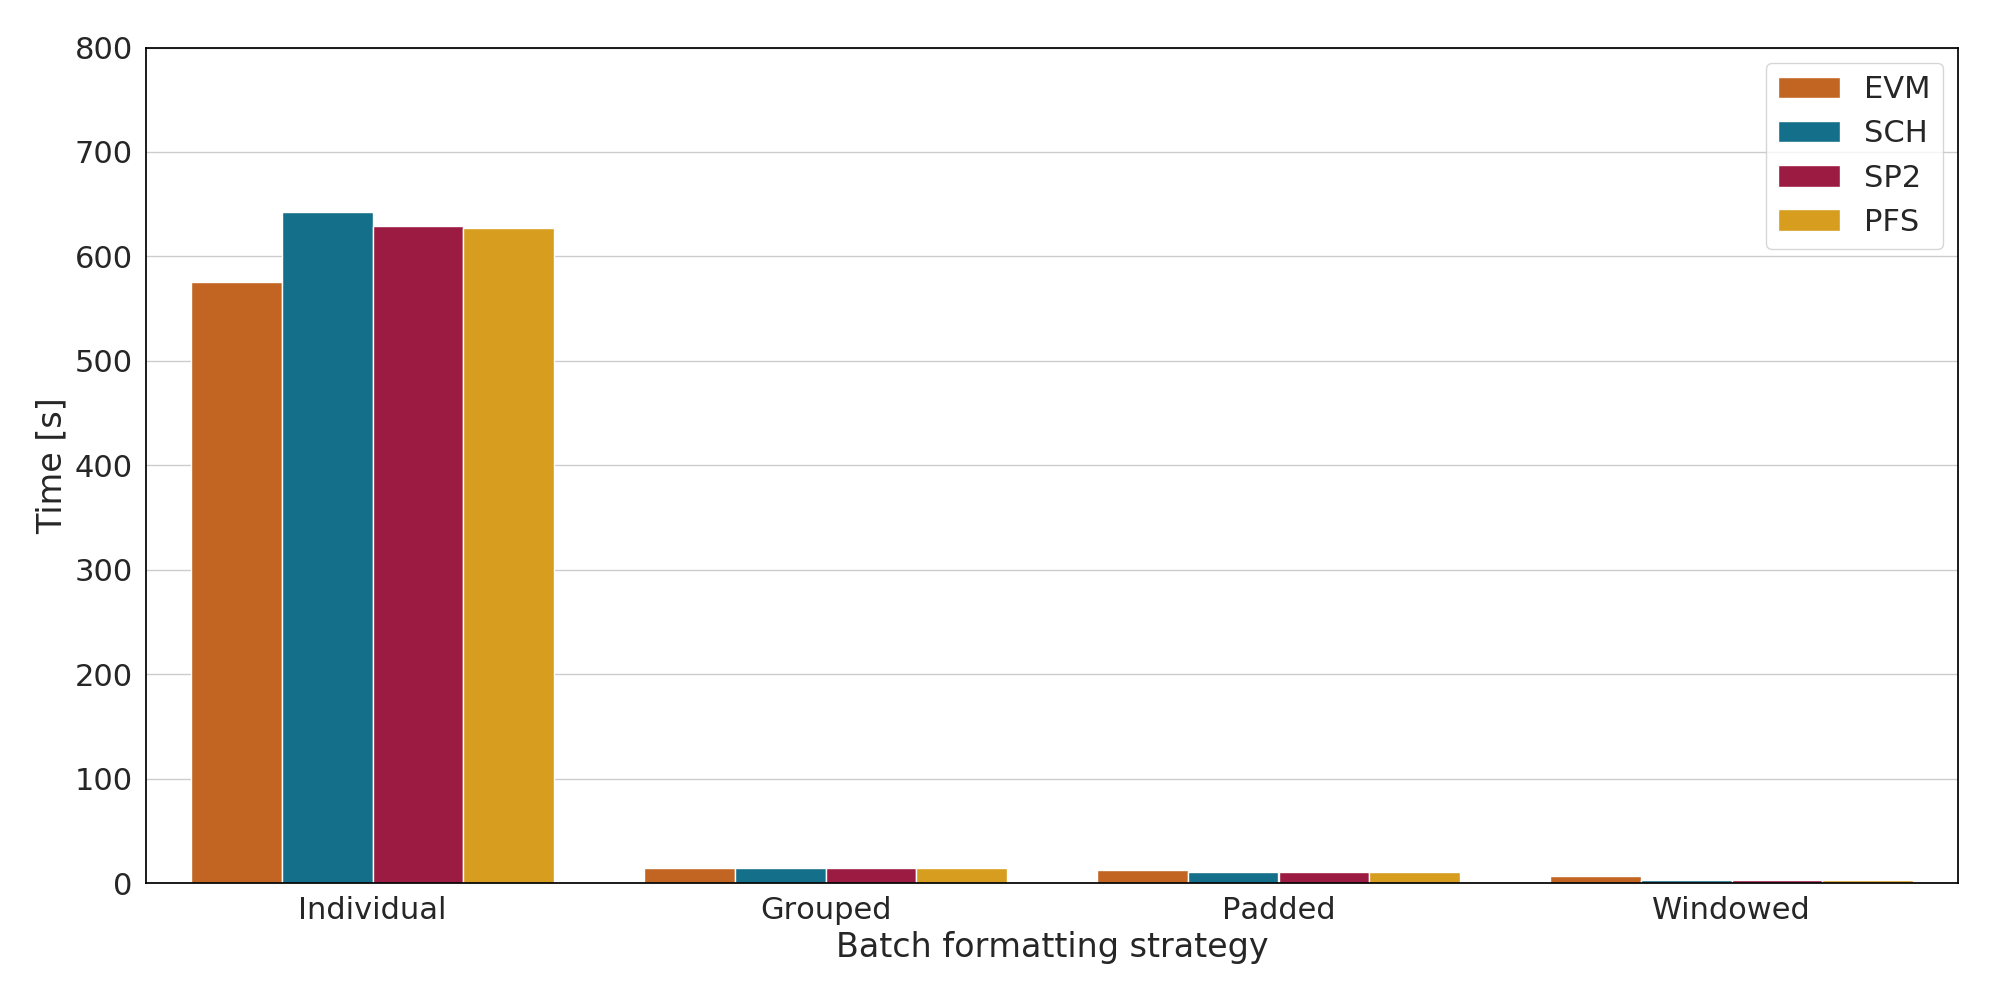
\includegraphics[width=\textwidth]{gfx/bpic2012/train_timings.png}
    \caption{Training times measured on BPIC12}
    \label{fig:BPIC12-training-timings}
\end{figure}
\begin{figure}
    \centering
    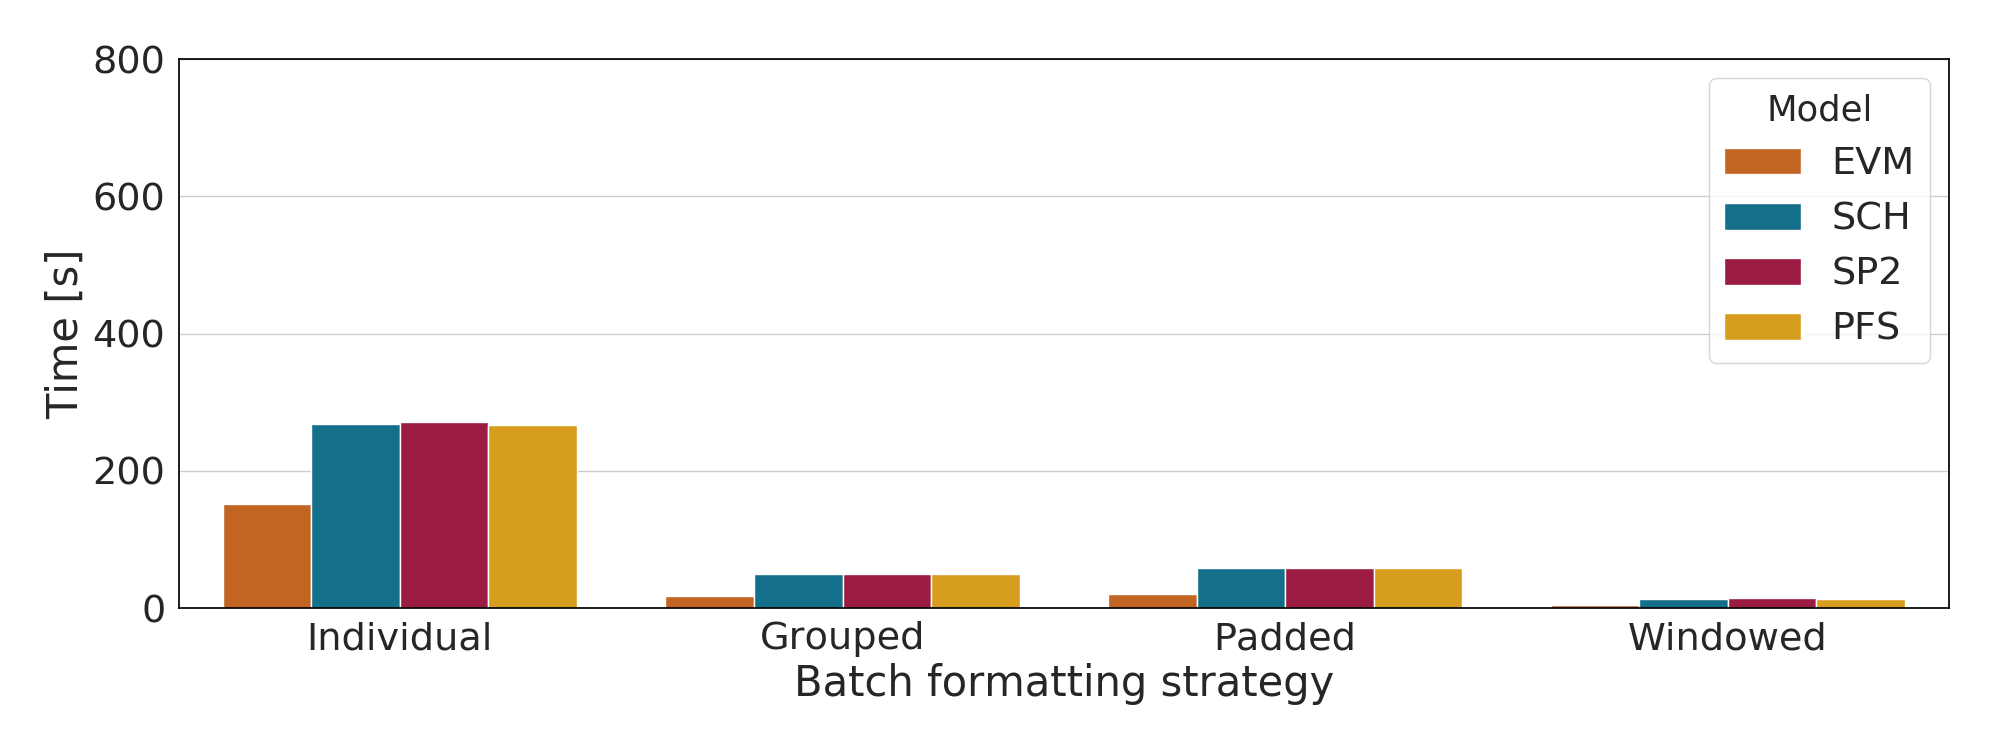
\includegraphics[width=\textwidth]{gfx/bpic2015_1/train_timings.png}
    \caption{Training times measured on BPIC15-1}
    \label{fig:BPIC15-1-training-timings}
\end{figure}
\begin{figure}
    \centering
    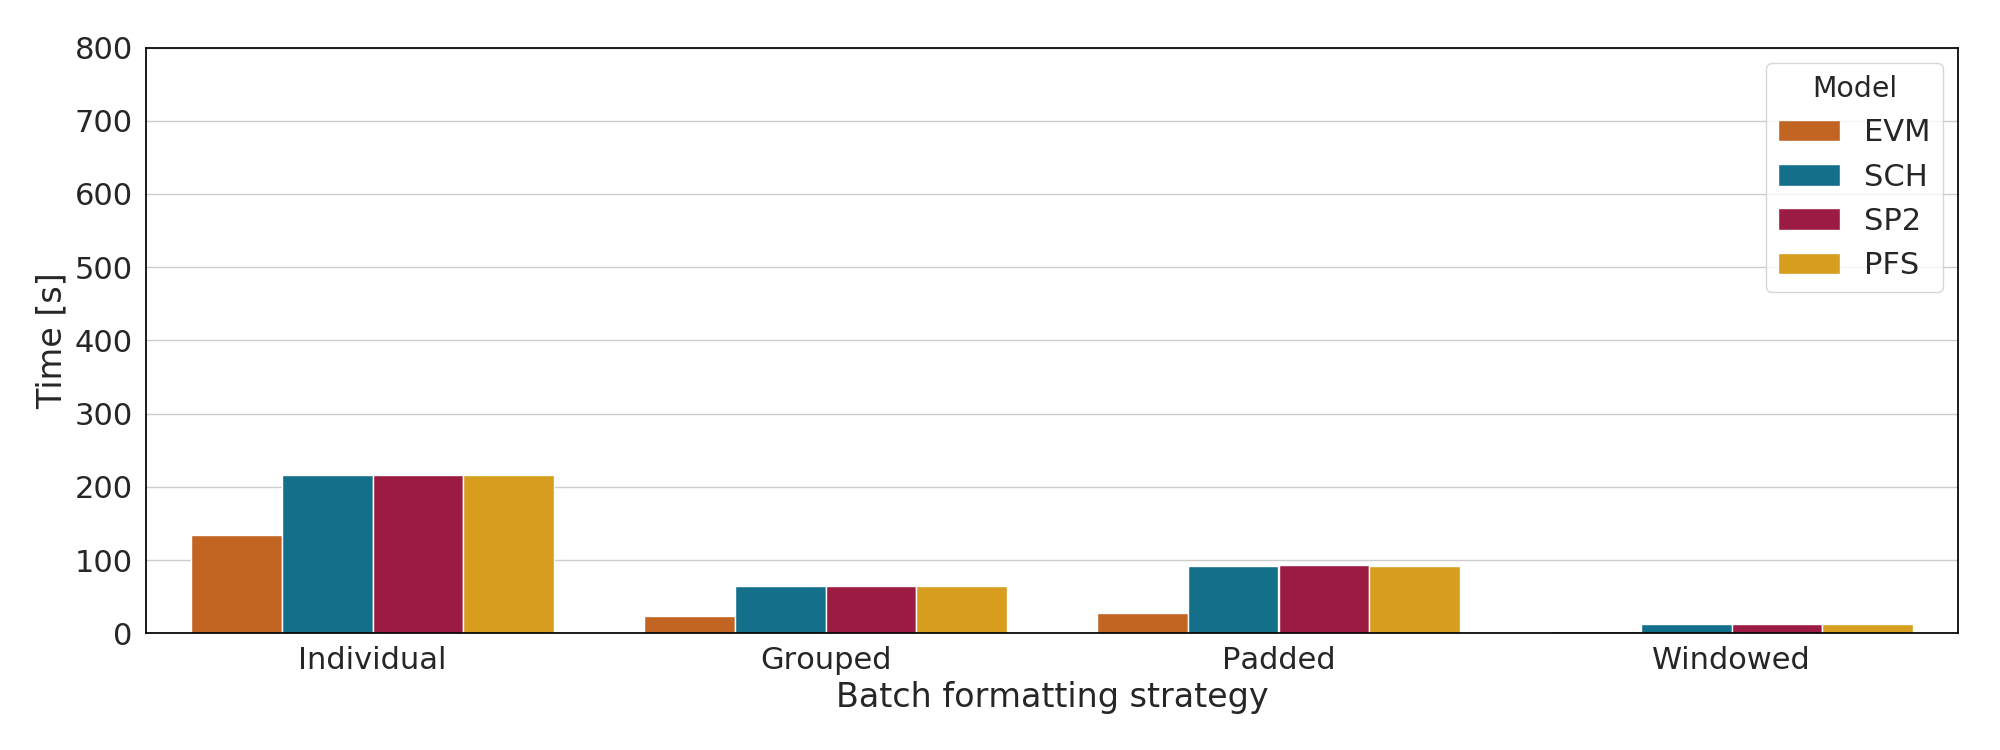
\includegraphics[width=\textwidth]{gfx/bpic2015_2/train_timings.png}
    \caption{Training times measured on BPIC15-2}
    \label{fig:BPIC15-2-training-timings}
\end{figure}
\begin{figure}
    \centering
    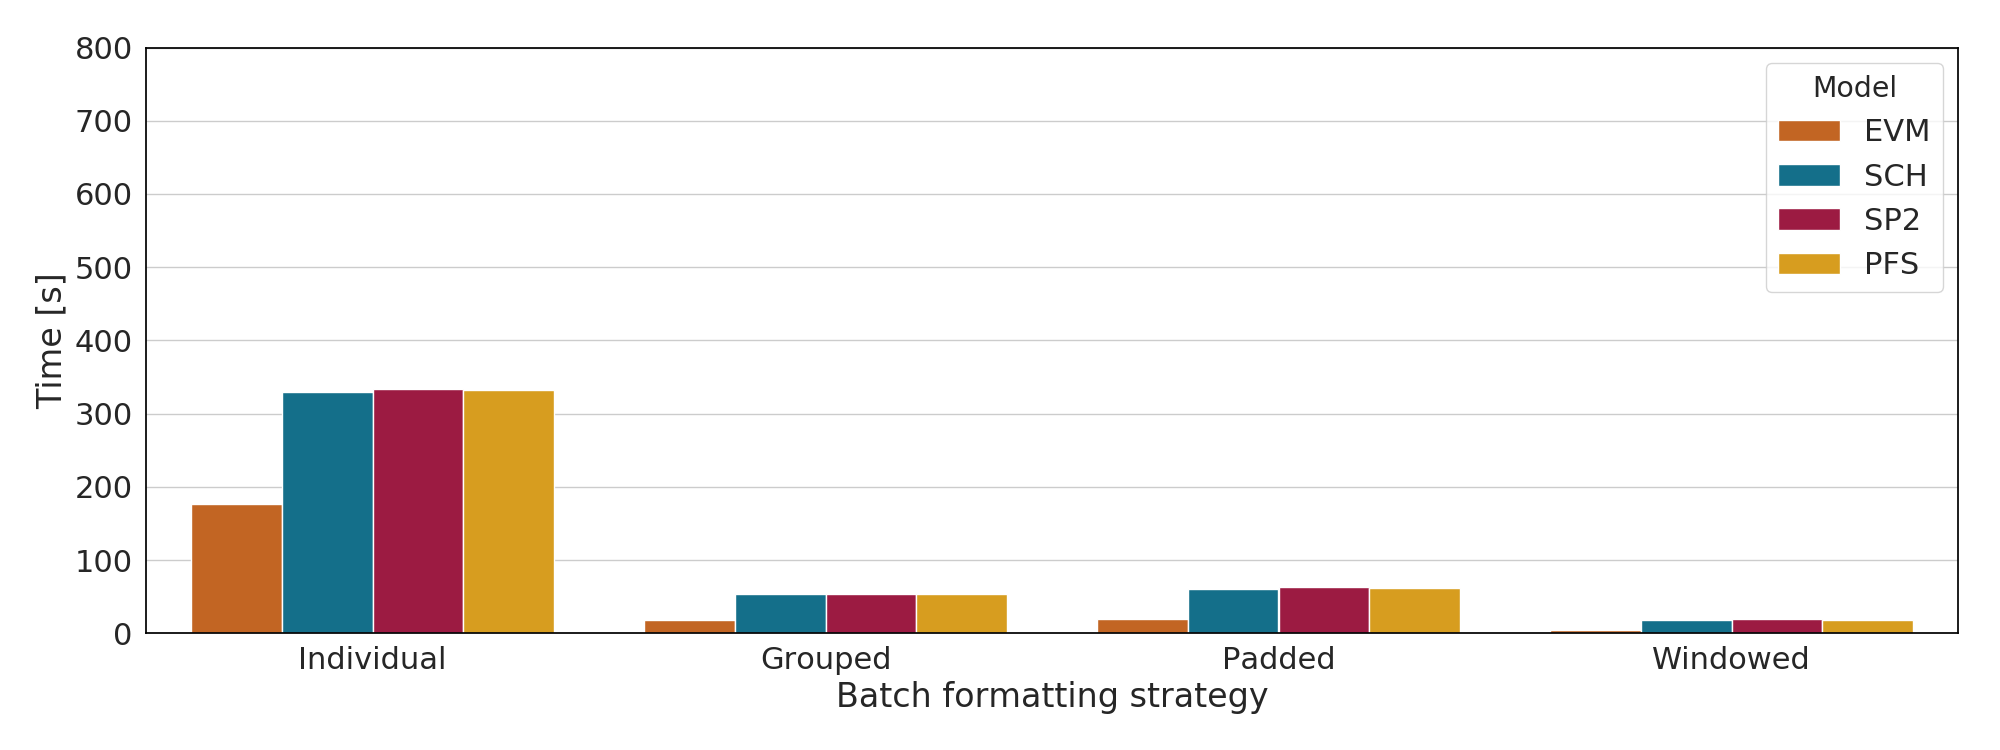
\includegraphics[width=\textwidth]{gfx/bpic2015_3/train_timings.png}
    \caption{Training times measured on BPIC15-3}
    \label{fig:BPIC15-3-training-timings}
\end{figure}
\begin{figure}
    \centering
    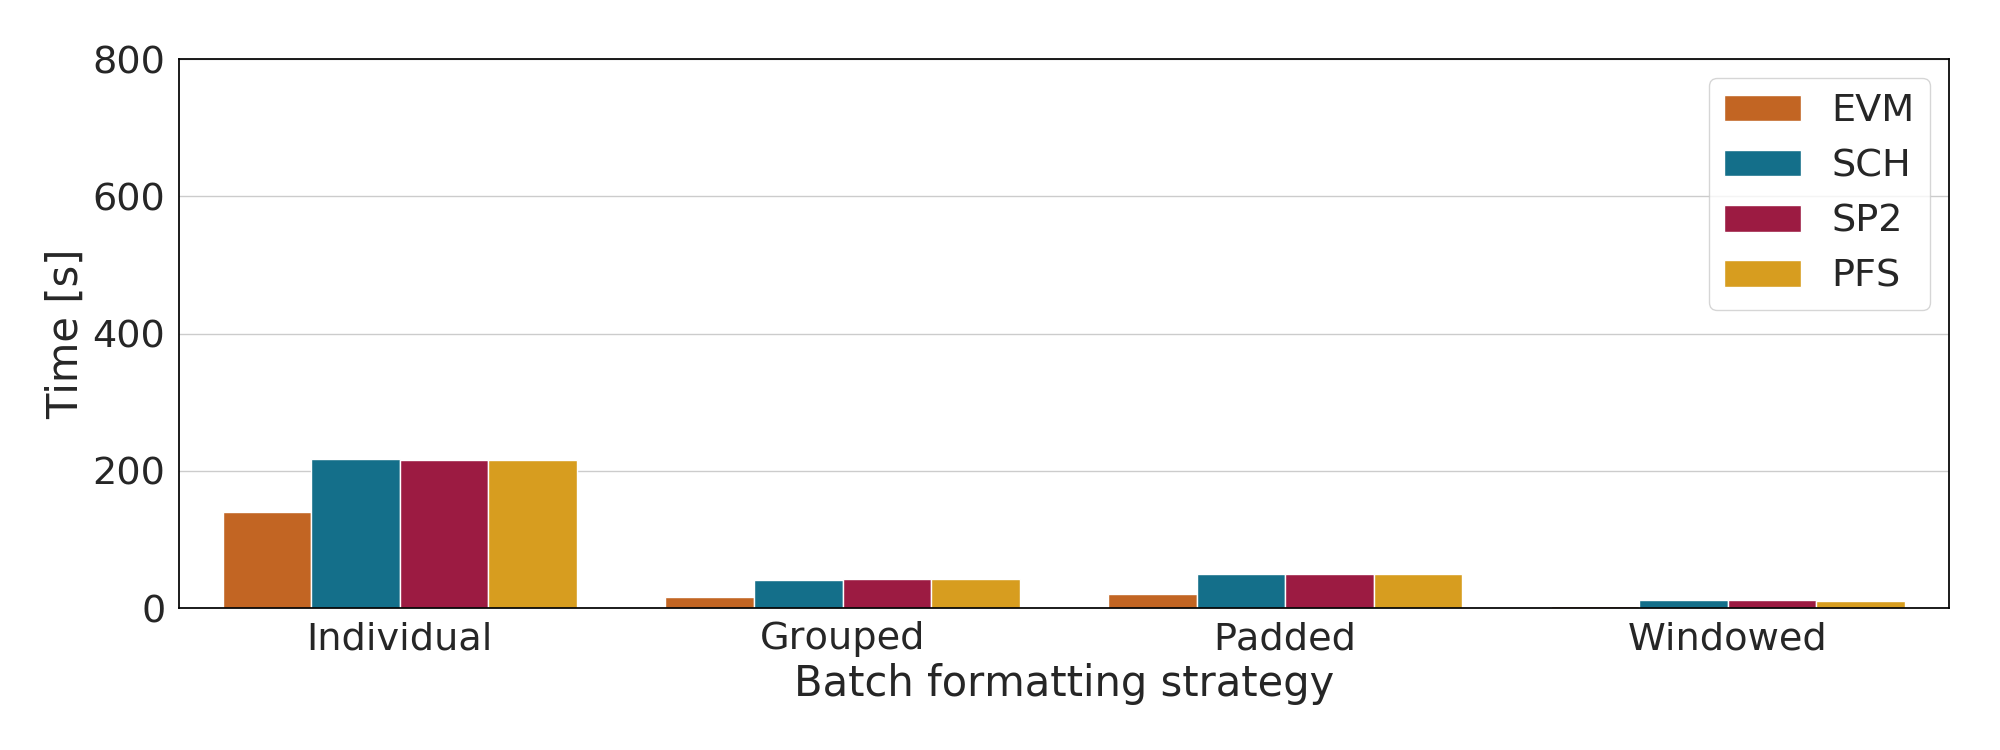
\includegraphics[width=\textwidth]{gfx/bpic2015_4/train_timings.png}
    \caption{Training times measured on BPIC15-4}
    \label{fig:BPIC15-4-training-timings}
\end{figure}
\begin{figure}
    \centering
    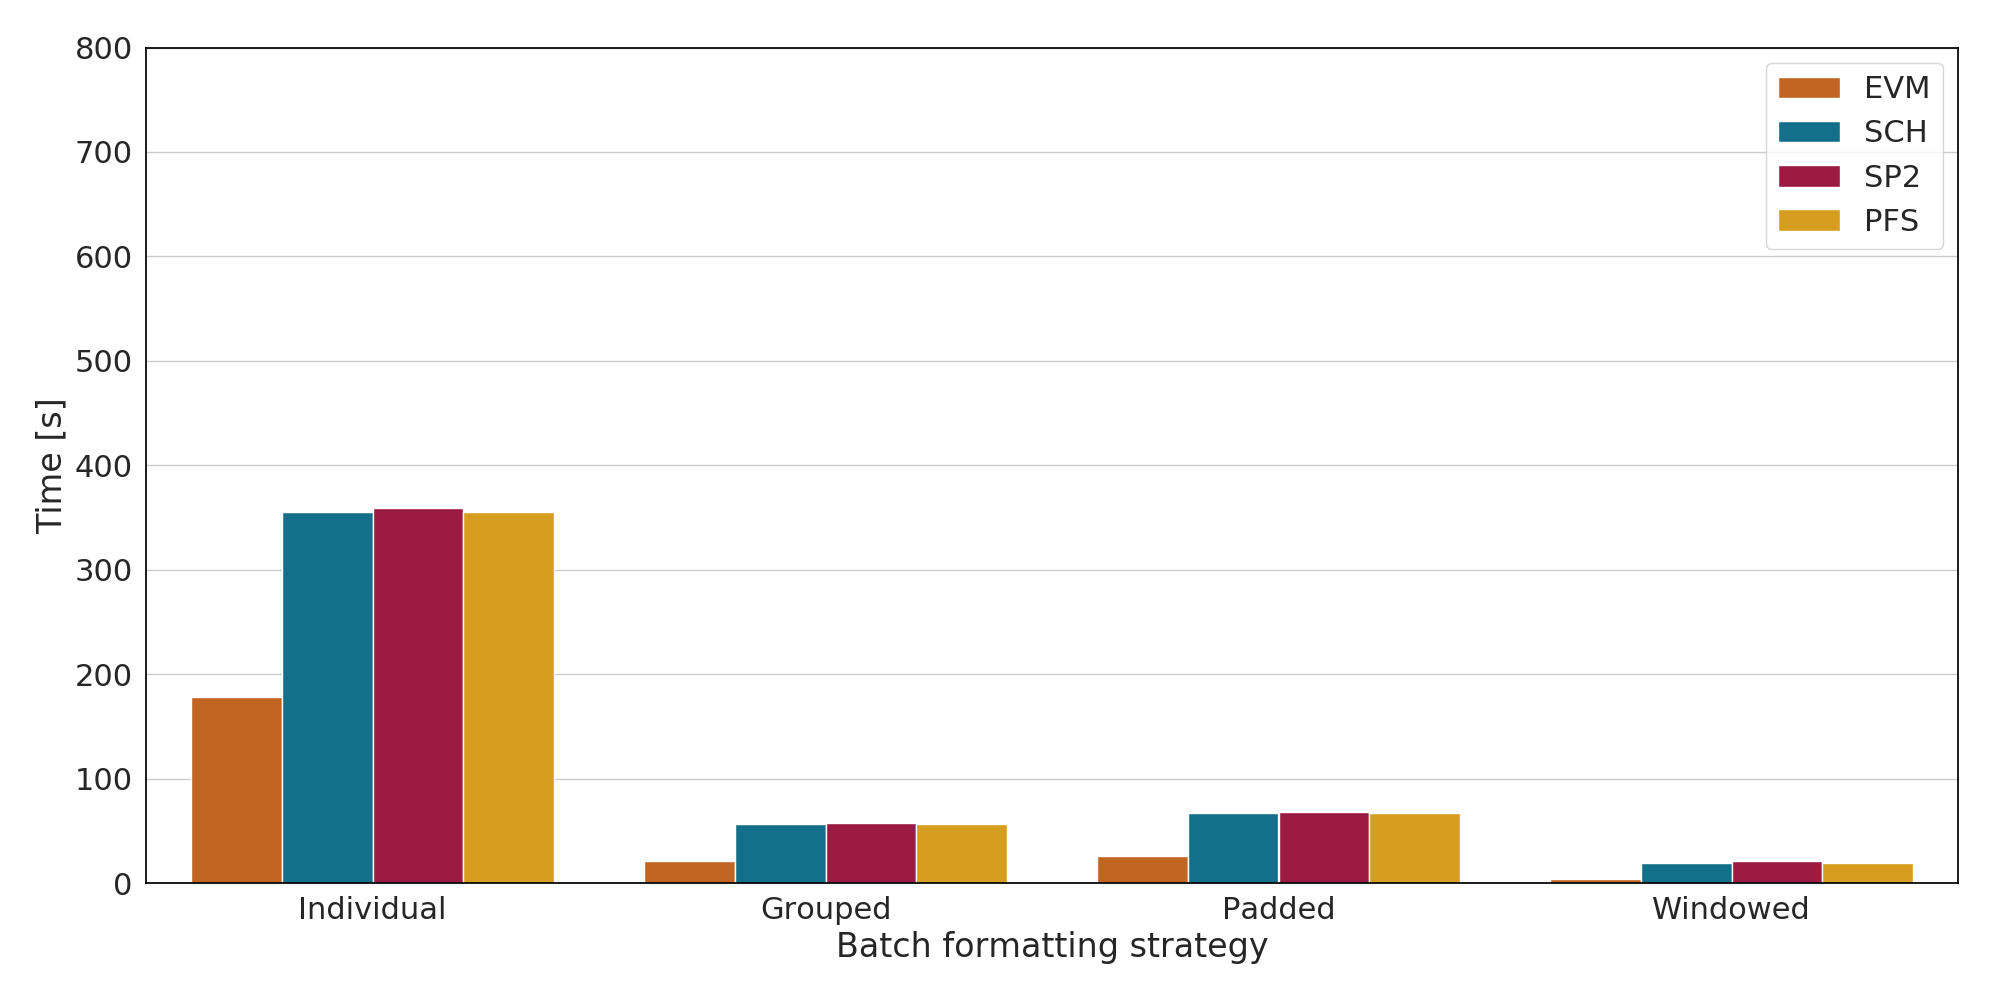
\includegraphics[width=\textwidth]{gfx/bpic2015_5/train_timings.png}
    \caption{Training times measured on BPIC15-5}
    \label{fig:BPIC15-5-training-timings}
\end{figure}
\FloatBarrier

\subsection*{Stability}
As we stressed in the introduction, the stability of a prediction model along the progress of a case greatly impacts the level of trust that users put into the model~\cite{metzger2015}. \autoref{appendix:evaluation-measurements} contains the figures that illustrate the stability of each model per batching strategy, grouped by dataset. Each figure for a batching strategy and a dataset contains four curves, one for each model. The curves show the model accuracy along the progression of all traces inside the validation set in steps of $5\%$. This subsection explains the results, again per batching strategy.\\

The individual batching strategy not only takes the most time, but it also leads to strong differences between the SCH, SP2, and PFS models. A good example is the difference between \autoref{fig:bpic15-3-individual-stability} and \autoref{fig:bpic15-3-grouped-stability}. In the latter figure, the SCH, SP2 and PFS curves are a lot closer to each other.

The grouping strategy increases the sample count per batch and this seems to have a harmonizing effect on the results as evidenced by the corresponding figures of all datasets. This harmonizing effect can be witnessed in the reduction of the standard deviation of the best accuracies of the SCH, SP2 and PFS models in \autoref{fig:grouping-accuracy-harmonization}.

\begin{figure}
    \centering
    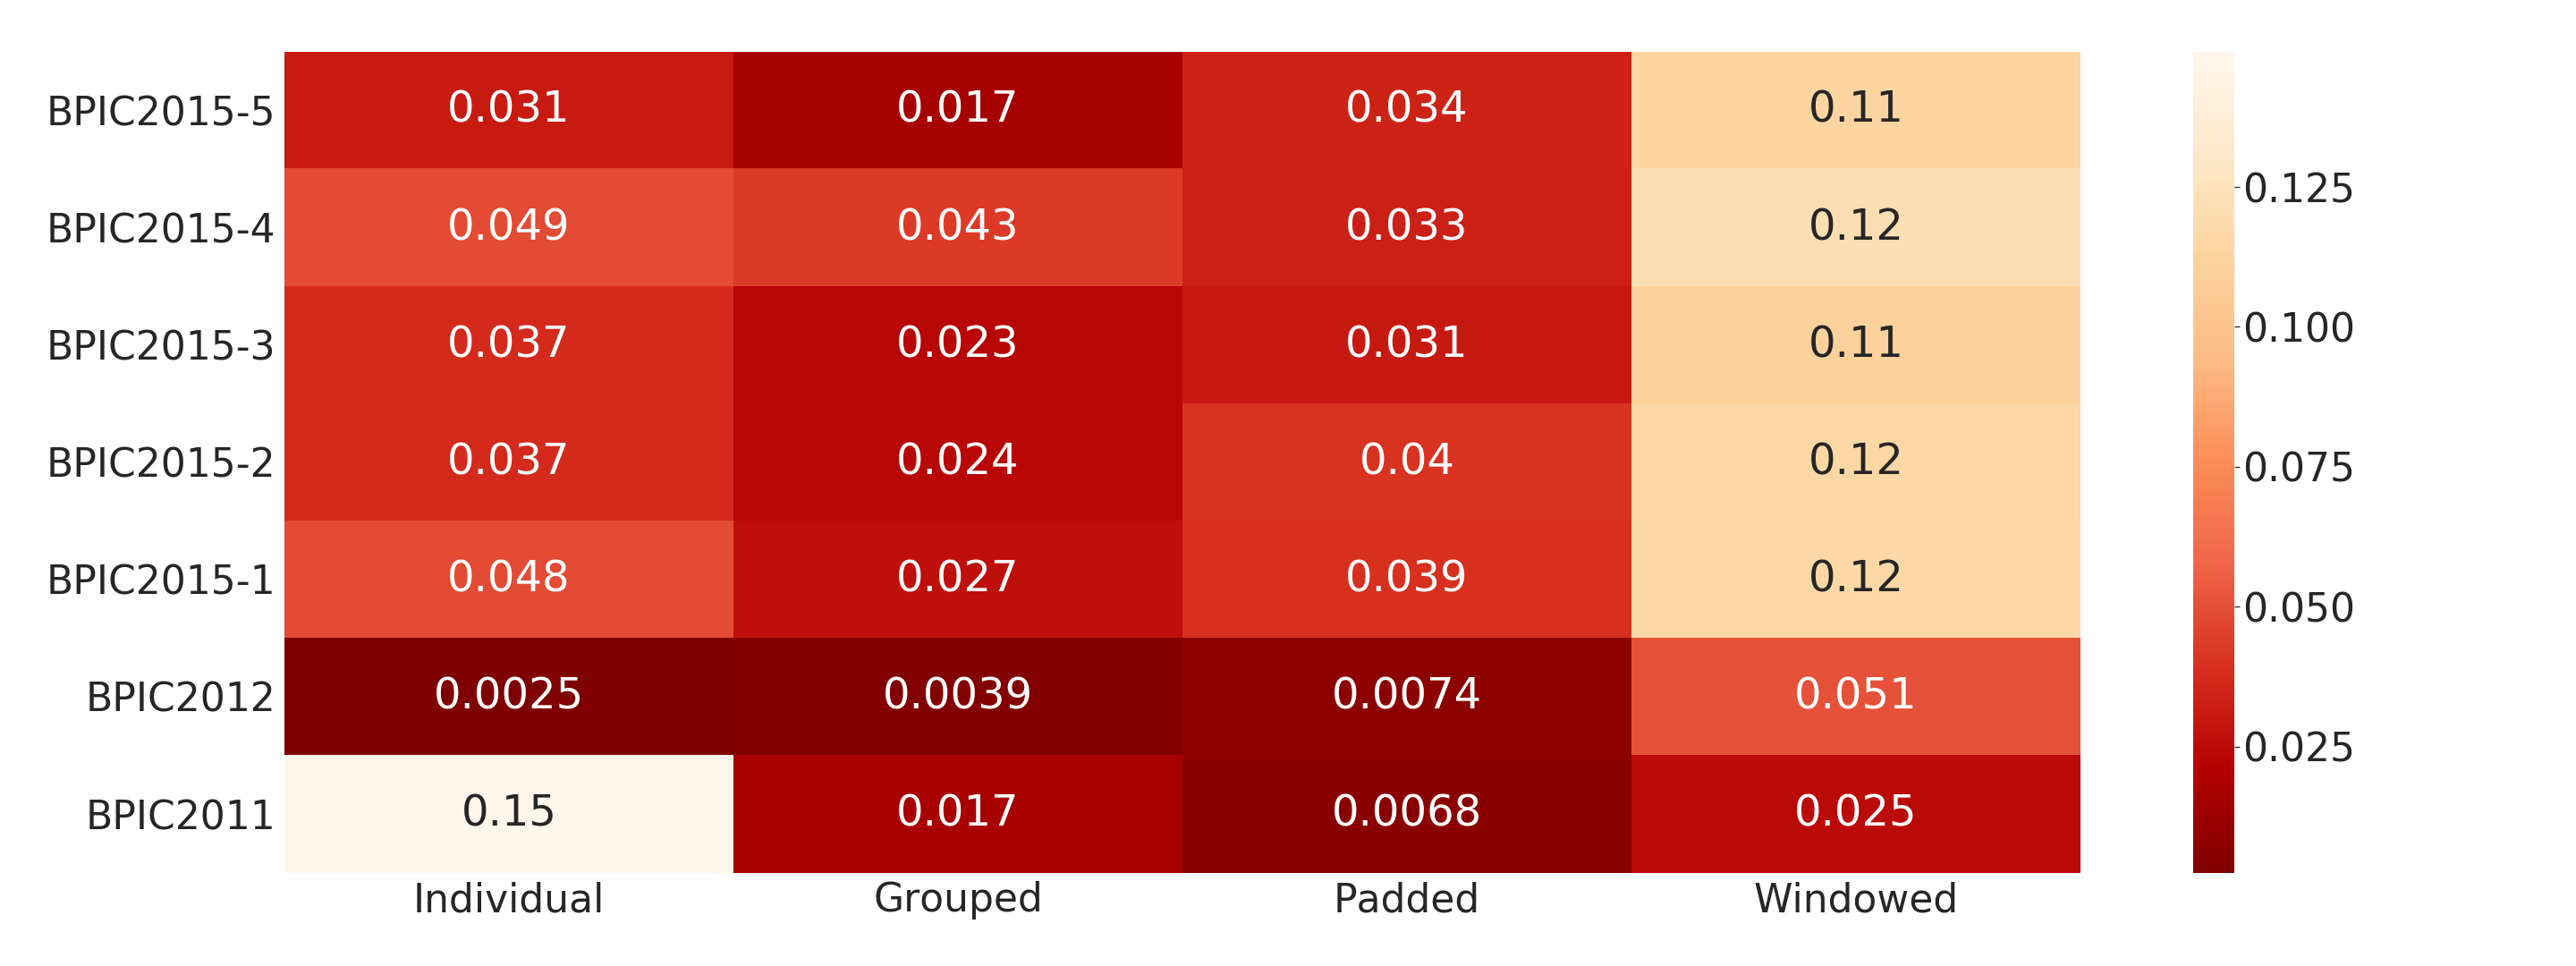
\includegraphics[width=\textwidth]{gfx/grouping-accuracy-harmonization.png}
    \caption[Batching strategy harmonizes top accuracies]{The grouping strategy often reduces the standard deviation between the highest accuracies of SCH, SP2 and PFS models}
    \label{fig:grouping-accuracy-harmonization}
\end{figure}

The padded strategy yields results very similar to the grouped strategy, with the exception of BPIC11. In this case, the training data had to be trimmed because the padded traces had required too much memory.

Klinkmüller et al. state that the windowing strategy leads to unstable results~\cite{klinkmuller2018reliablemonitoring}. While this statement seems to be especially true for the longer processes in BPIC11 and BPIC15, the windowing strategy seems to have less of an impact with shorter processes as evidenced with BPIC12. There, all models show a dip towards the end of the trace.\\

Generally, models were expected to become more accurate as the trace neared its end. However, this did not turn out to be the case. Instead, the accuracy was high when variability in the respective stage of the process was low. For example, processes in BPIC11 always begin similarly, as patients need to be onboarded~\cite{bose2011analysis}. This could be a cause for the high accuracies in the beginning. The processes in BPIC12 always end either on an approval or a dismissal of the application, making the models very accurate~\cite{adriansyah2012mining} in this stage.

\section{Discussion}\label{sec:eval:discussion}
After presenting and explaining our findings, we summarize our learnings in this section and compare our findings to the papers mentioned in \autoref{sec:eval:dataset-choice}.\\

First, we were able to confirm Klinkmüller et al.~\cite{klinkmuller2018reliablemonitoring} and their suspicion that windowed batching does not work well for sequence prediction. While it may be a performant strategy to use for time-series prediction, it does not work very well for predicting the future of a single case.

Secondly, we find that the grouping strategy frequently delivers the best results in terms of speed and accuracy. We realized that it should be iterated upon to include a threshold which limits batches to a maximum size and splits the larger batches accordingly. As evidenced by the charts, the grouping strategy seems to perform better with a medium to highly complex processes from BPIC11 and BPIC15, while padding works better with the simpler process from BPIC12. In combination with the SP2 model, the strategy contributed to most of the highest accuracies.

Third and lastly, we realize that Embeddings might not be useful on the currently available datasets as these might simply be too small. The lacking performance of the EVM model and its barely converging loss indicate that this might be the case. All accuracy/loss curves from training are enclosed in \autoref{appendix:loss-curves}, and show that especially for the EVM model, the loss optimization does not work properly.\\

We end the evaluation with a comparison of our best results with the initially mentioned publications based on BPIC12. While Tax et al.~\cite{tax2017} and Evermann et al.~\cite{evermann2016} were able to obtain an accuracy of $0.76$ and $0.768$ respectively, they did not focus on specific cases. Furthermore, Evermann et al. did not use Keras on top of Tensorflow but Tensorflow directly, which enabled him to directly make use of low-level functions. To the best of our knowledge, our implementation sufficiently approximates theirs, but this can be a reason for the bad results. Another very probable reason is their feature engineering~\cite{evermann2016}.

Böhmer et al.~\cite{boehmer2018probability} are able to attain an accuracy of $0.77$ with their statistical approach. While they argue that machine learning methods may perform better, they place great value on comprehensible reasoning information from the model.

Using the padding strategy, all SCH, SP2, and PFS score above $0.80$, with the SP2 model edging to the best accuracy of $0.82$. This supports the thesis by Böhmer et al. of lower comprehensibility at higher accuracy.
